%                **** IMPORTANT NOTICE *****
% This LaTeX file has been automatically produced by ProTeX v. 1.1
% Any changes made to this file will likely be lost next time
% this file is regenerated from its source. Send questions 
% to Arlindo da Silva, dasilva@gsfc.nasa.gov
 
\setlength{\oldparskip}{\parskip}
\setlength{\parskip}{1.5ex}
\setlength{\oldparindent}{\parindent}
\setlength{\parindent}{0pt}
\setlength{\oldbaselineskip}{\baselineskip}
\setlength{\baselineskip}{11pt}
 
%--------------------- SHORT-HAND MACROS ----------------------
\def\bv{\begin{verbatim}}
\def\ev{\end{verbatim}}
\def\be{\begin{equation}}
\def\ee{\end{equation}}
\def\bea{\begin{eqnarray}}
\def\eea{\end{eqnarray}}
\def\bi{\begin{itemize}}
\def\ei{\end{itemize}}
\def\bn{\begin{enumerate}}
\def\en{\end{enumerate}}
\def\bd{\begin{description}}
\def\ed{\end{description}}
\def\({\left (}
\def\){\right )}
\def\[{\left [}
\def\]{\right ]}
\def\<{\left  \langle}
\def\>{\right \rangle}
\def\cI{{\cal I}}
\def\diag{\mathop{\rm diag}}
\def\tr{\mathop{\rm tr}}
%-------------------------------------------------------------

\markboth{Left}{Source File: ESMF\_DistGridEx.F90,  Date: Tue May  5 20:59:41 MDT 2020
}

 
%/////////////////////////////////////////////////////////////

   \subsubsection{Single tile DistGrid with regular decomposition}
   
   The minimum information required to create an {\tt ESMF\_DistGrid} object
   for a single tile with default decomposition are the min and max of the tile
   in index space. The following call creates a DistGrid for a 
   1D index space tile with elements from 1 through 1000. 
%/////////////////////////////////////////////////////////////

 \begin{verbatim}
  distgrid = ESMF_DistGridCreate(minIndex=(/1/), maxIndex=(/1000/), rc=rc)
 
\end{verbatim}
 
%/////////////////////////////////////////////////////////////

   A default DELayout with 1 DE per PET will be created during the
   {\tt ESMF\_DistGridCreate()} call. The 1000 elements of the specified 1D tile
   are then block decomposed into the available DEs, and distributed across the
   PETs (same number as DEs by default).
   Assuming execution on 4 PETs, the (min) $\sim$ (max) indices of the DE-local
   blocks will be:
   \begin{verbatim}
     DE 0 - (1) ~ (250)
     DE 1 - (251) ~ (500)
     DE 2 - (501) ~ (750)
     DE 3 - (751) ~ (1000)
   \end{verbatim}
  
   DistGrids with rank > 1 can also be created with default decompositions,
   specifying only the min and max indices of the tile. The following creates a
   2D DistGrid for a 5x5 tile with default decomposition. 
%/////////////////////////////////////////////////////////////

 \begin{verbatim}
  distgrid = ESMF_DistGridCreate(minIndex=(/1,1/), maxIndex=(/5,5/), rc=rc)
 
\end{verbatim}
 
%/////////////////////////////////////////////////////////////

   The default decomposition for a DistGrid of rank $N$ will be $ (nDEs \times 1
   \times ... \times 1) $, where $nDEs$ is the number of DEs in the DELayout
   and there are $N-1$ factors of $1$. For the 2D example above this means
   a $4 \times 1$ regular decomposition if executed on 4 PETs and will result
   in the following DE-local LR regions:
   \begin{verbatim}
     DE 0 - (1,1) ~ (2,5)
     DE 1 - (3,1) ~ (3,5)
     DE 2 - (4,1) ~ (4,5)
     DE 3 - (5,1) ~ (5,5)
   \end{verbatim}
  
   In many cases the default decomposition will not suffice for higher rank
   DistGrids (rank > 1). For this reason a decomposition descriptor 
   {\tt regDecomp} argument is available during {\tt ESMF\_DistGridCreate()}. The
   following call creates a DistGrid on the same 2D tile as before, but now with
   a user specified regular decomposition of $2 \times 3 = 6 $ DEs. 
%/////////////////////////////////////////////////////////////

 \begin{verbatim}
  distgrid = ESMF_DistGridCreate(minIndex=(/1,1/), maxIndex=(/5,5/), &
    regDecomp=(/2,3/), rc=rc)
 
\end{verbatim}
 
%/////////////////////////////////////////////////////////////

   The default DE labeling sequence follows column major order for the
   {\tt regDecomp} argument:
   \begin{verbatim}
     -----------> 2nd dimension
     |  0  2  4
     |  1  3  5
     v
    1st dimension
   \end{verbatim}
  
   By default grid points along all dimensions are homogeneously divided between
   the DEs. The maximum element count difference between DEs along any dimension
   is 1. The (min) $\sim$ (max) indices of the DE-local blocks of the above
   example are as follows:
   \begin{verbatim}
     DE 0 - (1,1) ~ (3,2)
     DE 1 - (4,1) ~ (5,2)
     DE 2 - (1,3) ~ (3,4)
     DE 3 - (4,3) ~ (5,4)
     DE 4 - (1,5) ~ (3,5)
     DE 5 - (4,5) ~ (5,5)
   \end{verbatim}
   
   The specifics of the tile decomposition into DE-local LR domains can be
   modified by the optional {\tt decompflag} argument. The following line shows
   how this argument is used to keep ESMF's default decomposition in the first
   dimension but move extra grid points of the second dimension to the last DEs
   in that direction. Extra elements occur if the number of DEs for a certain
   dimension does not evenly divide its extent. In this example there are
   2 extra grid points for the second dimension because its extent is 5 but there
   are 3 DEs along this index space axis. 
%/////////////////////////////////////////////////////////////

 \begin{verbatim}
  distgrid = ESMF_DistGridCreate(minIndex=(/1,1/), maxIndex=(/5,5/), &
    regDecomp=(/2,3/), decompflag=(/ESMF_DECOMP_BALANCED, &
    ESMF_DECOMP_RESTLAST/), rc=rc)
 
\end{verbatim}
 
%/////////////////////////////////////////////////////////////

   Now DE 4 and DE 5 will hold the extra elements along the 2nd dimension.
   \begin{verbatim}
     DE 0 - (1,1) ~ (3,1)
     DE 1 - (4,1) ~ (5,1)
     DE 2 - (1,2) ~ (3,2)
     DE 3 - (4,2) ~ (5,2)
     DE 4 - (1,3) ~ (3,5)
     DE 5 - (4,3) ~ (5,5)
   \end{verbatim}
  
   An alternative way of indicating the DE-local LR regions is to list the 
   index space coordinate as given by the associated DistGrid tile for each
   dimension. For this 2D example there are two lists (dim 1) / (dim 2) for each
   DE:
   \begin{verbatim}
     DE 0 - (1,2,3) / (1)
     DE 1 - (4,5)   / (1)
     DE 2 - (1,2,3) / (2)
     DE 3 - (4,5)   / (2)
     DE 4 - (1,2,3) / (3,4,5)
     DE 5 - (4,5)   / (3,4,5)
   \end{verbatim}
  
   Information about DE-local LR regions in the latter format can be obtained 
   from the DistGrid object by use of {\tt ESMF\_DistGridGet()} methods:
   
%/////////////////////////////////////////////////////////////

 \begin{verbatim}
  allocate(dimExtent(2, 0:5)) ! (dimCount, deCount)
  call ESMF_DistGridGet(distgrid, delayout=delayout, &
    indexCountPDe=dimExtent, rc=rc)
  if (rc /= ESMF_SUCCESS) call ESMF_Finalize(endflag=ESMF_END_ABORT)
  call ESMF_DELayoutGet(delayout, localDeCount=localDeCount, rc=rc)
  if (rc /= ESMF_SUCCESS) call ESMF_Finalize(endflag=ESMF_END_ABORT)
  allocate(localDeToDeMap(0:localDeCount-1))
  call ESMF_DELayoutGet(delayout, localDeToDeMap=localDeToDeMap, rc=rc)
  if (rc /= ESMF_SUCCESS) call ESMF_Finalize(endflag=ESMF_END_ABORT)
  do localDe=0, localDeCount-1
    de = localDeToDeMap(localDe)
    do dim=1, 2
      allocate(localIndexList(dimExtent(dim, de))) ! allocate list 
                                                   ! to hold indices
      call ESMF_DistGridGet(distgrid, localDe=localDe, dim=dim, &
        indexList=localIndexList, rc=rc)
      if (rc /= ESMF_SUCCESS) call ESMF_Finalize(endflag=ESMF_END_ABORT)
      print *, "local DE ", localDe," - DE ",de, &
        " localIndexList along dim=", dim," :: ", localIndexList
      deallocate(localIndexList)
    enddo
  enddo
  deallocate(localDeToDeMap)
  deallocate(dimExtent)
 
\end{verbatim}
 
%/////////////////////////////////////////////////////////////

   The advantage of the {\tt localIndexList} format over the minIndex/maxIndex 
   format is that it can be used directly for DE-local to tile index 
   dereferencing. Furthermore the {\tt localIndexList} allows to express very
   general decompositions such as the cyclic decompositions in the first
   dimension generated by the following call: 
%/////////////////////////////////////////////////////////////

 \begin{verbatim}
  distgrid = ESMF_DistGridCreate(minIndex=(/1,1/), maxIndex=(/5,5/), &
    regDecomp=(/2,3/), &
    decompflag=(/ESMF_DECOMP_CYCLIC,ESMF_DECOMP_RESTLAST/), rc=rc)
 
\end{verbatim}
 
%/////////////////////////////////////////////////////////////

   with decomposition:
   \begin{verbatim}
     DE 0 - (1,3,5) / (1)
     DE 1 - (2,4)   / (1)
     DE 2 - (1,3,5) / (2)
     DE 3 - (2,4)   / (2)
     DE 4 - (1,3,5) / (3,4,5)
     DE 5 - (2,4)   / (3,4,5)
   \end{verbatim}
  
   Finally, a DistGrid object is destroyed by calling 
%/////////////////////////////////////////////////////////////

 \begin{verbatim}
  call ESMF_DistGridDestroy(distgrid, rc=rc)
 
\end{verbatim}
 
%/////////////////////////////////////////////////////////////

   \subsubsection{DistGrid and DELayout}
   
   The examples of this section use the 2D DistGrid of the previous section 
   to show the interplay between DistGrid and DELayout. By default, i.e.
   without specifying the {\tt delayout} argument, a DELayout will be created
   during DistGrid creation that provides as many DEs as the DistGrid
   object requires. The implicit call to {\tt ESMF\_DELayoutCreate()} is issued
   with a fixed number of DEs and default settings in all other aspects. The
   resulting DE to PET mapping depends on the number of PETs of the current VM
   context. Assuming 6 PETs in the VM 
%/////////////////////////////////////////////////////////////

 \begin{verbatim}
  distgrid = ESMF_DistGridCreate(minIndex=(/1,1/), maxIndex=(/5,5/), &
    regDecomp=(/2,3/), rc=rc)
 
\end{verbatim}
 
%/////////////////////////////////////////////////////////////

   will result in the following domain decomposition in terms of DEs
   \begin{verbatim}
     0  2  4
     1  3  5
   \end{verbatim}
   and their layout or distribution over the available PETs:
   \begin{verbatim}
     DE 0  -> PET 0
     DE 1  -> PET 1
     DE 2  -> PET 2
     DE 3  -> PET 3
     DE 4  -> PET 4
     DE 5  -> PET 5
   \end{verbatim}
   
   Running the same example on a 4 PET VM will not change the domain 
   decomposition into 6 DEs as specified by
   \begin{verbatim}
     0  2  4
     1  3  5
   \end{verbatim}
   but the layout across PETs will now contain multiple DE-to-PET mapping with 
   default cyclic distribution:
   \begin{verbatim}
     DE 0  -> PET 0
     DE 1  -> PET 1
     DE 2  -> PET 2
     DE 3  -> PET 3
     DE 4  -> PET 0
     DE 5  -> PET 1
   \end{verbatim}
  
   Sometimes it may be desirable for performance tuning to construct a DELayout
   with specific characteristics. For instance, if the 6 PETs of the above 
   example are running on 3 nodes of a dual-SMP node cluster and there is a 
   higher communication load along the first dimension of the model than along 
   the second dimension it would be sensible to place DEs according to this 
   knowledge. 
%/////////////////////////////////////////////////////////////

   The following example first creates a DELayout 
   with 6 DEs where groups of 2 DEs are to be in fast connection. This DELayout 
   is then used to create a DistGrid. 
%/////////////////////////////////////////////////////////////

 \begin{verbatim}
  delayout = ESMF_DELayoutCreate(deCount=6, deGrouping=(/(i/2,i=0,5)/), rc=rc)
 
\end{verbatim}
 
%/////////////////////////////////////////////////////////////

 \begin{verbatim}
  distgrid = ESMF_DistGridCreate(minIndex=(/1,1/), maxIndex=(/5,5/), &
    regDecomp=(/2,3/), delayout=delayout, rc=rc)
 
\end{verbatim}
 
%/////////////////////////////////////////////////////////////

   This will ensure a distribution of DEs across the cluster resource 
   in the following way:
   \begin{verbatim}
     0   2   4
     1   3   5
    SMP SMP SMP
   \end{verbatim}
   
   The interplay between DistGrid and DELayout may at first seem complicated.
   The simple but important rule to understand is that DistGrid describes a 
   domain decomposition and each domain is labeled with a DE number. The DELayout
   describes how these DEs are laid out over the compute resources of the VM, 
   i.e. PETs. The DEs are purely logical elements of decomposition and may be 
   relabeled to fit the algorithm or legacy code better. The following 
   example demonstrates this by describing the exact same distribution of the 
   domain data across the fictitious cluster of SMP-nodes with a different 
   choice of DE labeling: 
%/////////////////////////////////////////////////////////////

 \begin{verbatim}
  delayout = ESMF_DELayoutCreate(deCount=6, deGrouping=(/(mod(i,3),i=0,5)/), &
    rc=rc)
 
\end{verbatim}
 
%/////////////////////////////////////////////////////////////

 \begin{verbatim}
  distgrid = ESMF_DistGridCreate(minIndex=(/1,1/), maxIndex=(/5,5/), &
    regDecomp=(/2,3/), deLabelList=(/0,3,1,4,2,5/), delayout=delayout, rc=rc)
 
\end{verbatim}
 
%/////////////////////////////////////////////////////////////

   Here the {\tt deLabelList} argument changes the default DE label sequence from
   column major to row major. The DELayout compensates for this change in DE
   labeling by changing the {\tt deGrouping} argument to map the first dimension
   to SMP nodes as before. The decomposition and layout now looks as follows:
   \begin{verbatim}
     0   1   2
     3   4   5
    SMP SMP SMP
   \end{verbatim}
   
   Finally, in order to achieve a completely user-defined distribution of the
   domain data across the PETs of the VM a DELayout may be created from a
   {\tt petMap} before using it in the creation of a DistGrid. If for
   instance the desired distribution of a 2 x 3 decomposition puts the DEs of 
   the first row onto 3 separate PETs (PET 0, 1, 2) and groups the DEs of 
   the second row onto PET 3 a {\tt petMap} must first be setup that
   takes the DE labeling of the DistGrid into account.The following lines of 
   code result in the desired distribution using column major DE labeling by 
   first create a DELayout and then using it in the DistGrid creation. 
%/////////////////////////////////////////////////////////////

 \begin{verbatim}
  delayout = ESMF_DELayoutCreate(petMap=(/0,3,1,3,2,3/), rc=rc)
 
\end{verbatim}
 
%/////////////////////////////////////////////////////////////

 \begin{verbatim}
  distgrid = ESMF_DistGridCreate(minIndex=(/1,1/), maxIndex=(/5,5/), &
    regDecomp=(/2,3/), delayout=delayout, rc=rc)
 
\end{verbatim}
 
%/////////////////////////////////////////////////////////////

   This decomposes the global domain into
   \begin{verbatim}
     0   2   4
     1   3   5
   \end{verbatim}
   and associates the DEs to the following PETs:
   \begin{verbatim}
     DE 0  -> PET 0
     DE 1  -> PET 3
     DE 2  -> PET 1
     DE 3  -> PET 3
     DE 4  -> PET 2
     DE 5  -> PET 3
   \end{verbatim} 
%/////////////////////////////////////////////////////////////

   \subsubsection{Single tile DistGrid with decomposition by DE blocks}
   
   In the previous examples the DistGrid objects were created with regular
   decompositions. In some cases a regular decomposition may not be the most
   natural choice to decompose and distribute the index space. The 
   DE block version of {\tt ESMF\_DistGridCreate()} offers more control
   over the precise decomposition. The following example shows how the 
   {\tt deBlockList} argument is used to determine exactly what index space
   block ends up on each DE.
  
   A single 5x5 tile is decomposed into 6 DEs. To this end a list is
   constructed that holds the min and max indices of all six DE
   blocks. The DE blocks must be constructed to cover the index space without
   overlapping each other. It is okay to leave holes in the index space, i.e.
   the DE blocks do not completely cover the index space tile. 
%/////////////////////////////////////////////////////////////

 \begin{verbatim}
  allocate(deBlockList(2, 2, 6))  ! (dimCount, 2, deCount)
  deBlockList(:,1,1) = (/1,1/)  ! minIndex  1st deBlock
  deBlockList(:,2,1) = (/3,2/)  ! maxIndex  1st deBlock
  deBlockList(:,1,2) = (/4,1/)  ! minIndex  2nd deBlock
  deBlockList(:,2,2) = (/5,2/)  ! maxIndex  2nd deBlock
  deBlockList(:,1,3) = (/1,3/)
  deBlockList(:,2,3) = (/2,4/)
  deBlockList(:,1,4) = (/3,3/)
  deBlockList(:,2,4) = (/5,4/)
  deBlockList(:,1,5) = (/1,5/)
  deBlockList(:,2,5) = (/3,5/)
  deBlockList(:,1,6) = (/4,5/)  ! minIndex  6th deBlock
  deBlockList(:,2,6) = (/5,5/)  ! maxInbex  6th deBlock
 
\end{verbatim}
 
%/////////////////////////////////////////////////////////////

 \begin{verbatim}
  distgrid = ESMF_DistGridCreate(minIndex=(/1,1/), maxIndex=(/5,5/), &
    deBlockList=deBlockList, rc=rc)
 
\end{verbatim}
 
%/////////////////////////////////////////////////////////////

   \subsubsection{2D multi-tile DistGrid with regular decomposition}
   
   Creating a DistGrid from a list of LR tiles is a straightforward
   extension of the single tile case. The first four 
   arguments of {\tt ESMF\_DistGridCreate()} are promoted to rank 2 where the 
   second dimension is the tile index.
   
   The following 2D multi-tile domain consisting of 3 LR tiles will 
   be used in the examples of this section:
   \begin{verbatim}
  
     ----------------------------------------> 2nd dim
     |
     |                   (1,11)-----(1,20)
     |                   |               | 
     |                   |               | 
     |                   |               | 
     |                   |               | 
     |                   |               | 
     |                   (10,11)---(10,20)
     |  (11,1)----(11,10)(11,11)---(11,20)
     |  |               ||               |
     |  |               ||               |
     |  |               ||               |
     |  |               ||               |
     |  |               ||               |
     |  (20,1)----(20,10)(20,11)---(20,20)
     |
     |
     v
    1st dim
   \end{verbatim}
  
   The first step in creating a multi-tile global domain is to construct the
   {\tt minIndex} and {\tt maxIndex} arrays. 
%/////////////////////////////////////////////////////////////

 \begin{verbatim}
  allocate(minIndexPTile(2,3))    ! (dimCount, tileCount)
  allocate(maxIndexPTile(2,3))    ! (dimCount, tileCount)
  minIndexPTile(:,1) = (/11,1/)
  maxIndexPTile(:,1) = (/20,10/)
  minIndexPTile(:,2) = (/11,11/)
  maxIndexPTile(:,2) = (/20,20/)
  minIndexPTile(:,3) = (/1,11/)
  maxIndexPTile(:,3) = (/10,20/)
 
\end{verbatim}
 
%/////////////////////////////////////////////////////////////

   Next the regular decomposition for each tile is set up in the
   {\tt regDecomp} array. In this example each tile is associated with a
   single DE. 
%/////////////////////////////////////////////////////////////

 \begin{verbatim}
  allocate(regDecompPTile(2,3))    ! (dimCount, tileCount)
  regDecompPTile(:,1) = (/1,1/)    ! one DE
  regDecompPTile(:,2) = (/1,1/)    ! one DE
  regDecompPTile(:,3) = (/1,1/)    ! one DE
 
\end{verbatim}
 
%/////////////////////////////////////////////////////////////

   Finally the DistGrid can be created by calling 
%/////////////////////////////////////////////////////////////

 \begin{verbatim}
  distgrid = ESMF_DistGridCreate(minIndexPTile=minIndexPTile, &
    maxIndexPTile=maxIndexPTile, regDecompPTile=regDecompPTile, rc=rc)
 
\end{verbatim}
 
%/////////////////////////////////////////////////////////////

   The default DE labeling sequence is identical to the tile labeling sequence
   and follows the sequence in which the tiles are defined during the create
   call. However, DE labels start at 0 whereas tile labels start at 1. In this 
   case the DE labels look as:
   \begin{verbatim}
           2
       0   1
   \end{verbatim}
  
   Each tile can be decomposed differently into DEs. The default DE labeling 
   follows the column major order for each tile. This is demonstrated in the
   following case where the multi-tile global domain is decomposed into 9 DEs, 
%/////////////////////////////////////////////////////////////

 \begin{verbatim}
  regDecompPTile(:,1) = (/2,2/)    ! 4 DEs
  regDecompPTile(:,2) = (/1,3/)    ! 3 DEs
  regDecompPTile(:,3) = (/2,1/)    ! 2 DEs
  
  distgrid = ESMF_DistGridCreate(minIndexPTile=minIndexPTile, &
    maxIndexPTile=maxIndexPTile, regDecompPTile=regDecompPTile, rc=rc)
 
\end{verbatim}
 
%/////////////////////////////////////////////////////////////

   resulting in the following decomposition:
   \begin{verbatim}
             +-------+
             |   7   |
             |       |
             |   8   |
     +-------+-------+
     | 0   2 |       |
     |       | 4 5 6 |
     | 1   3 |       |
     +-------+-------+
   \end{verbatim}
  
   \begin{verbatim}
     DE 0 - (11,1)  ~ (15,5)
     DE 1 - (16,1)  ~ (20,5)
     DE 2 - (11,6)  ~ (15,10)
     DE 3 - (16,6)  ~ (20,10)
     DE 4 - (11,11) ~ (20,14)
     DE 5 - (11,15) ~ (20,17)
     DE 6 - (11,18) ~ (20,20)
     DE 7 - (1,11)  ~ (5,20)
     DE 8 - (6,11)  ~ (10,20)
   \end{verbatim}
  
   The {\tt decompflag} and {\tt deLabelList} arguments can be used much like
   in the single LR domain case to overwrite the default grid decomposition 
   (per tile) and to change the overall DE labeling sequence, respectively. 
%/////////////////////////////////////////////////////////////

   \subsubsection{Arbitrary DistGrids with user-supplied sequence indices}
   \label{DistGrid:ArbitrarySeqInd}
  
   The third, and most flexible way of creating an ESMF DistGrid object is
   by specifying the arbitrary sequence indices of all the index space elements
   associated with a particular DE. The concept of sequence index
   comes into the DistGrid class through the support it implements for the 
   communication methods of higher classes: Arrays and Fields. This support
   is based by associating a unique {\em sequence index} with each
   DistGrid index tuple. The sequence index can be used to address every Array
   or Field element. By default, the DistGrid does not actually generate and
   store the sequence index of each element. Instead a default sequence through
   the elements is implemented in the DistGrid code. This default sequence 
   is used internally when needed.
  
   The DistGrid class provides two {\tt ESMF\_DistGridCreate()} calls that 
   allow the user to specify arbitrary sequence indices, overriding the use of
   the default sequence index scheme. The user sequence indices are passed to
   the DistGrid in form of 1d Fortran arrays, one array on each PET. The local
   size of this array on each PET determines the number of DistGrid elements on
   the PET. The supplied sequence indices must be unique across all PETs. 
   
%/////////////////////////////////////////////////////////////

 \begin{verbatim}
  allocate(arbSeqIndexList(10))   ! each PET will have 10 elements
  
  do i=1, 10
    arbSeqIndexList(i) = (i-1)*petCount + localPet ! initialize unique 
                                                   ! seq. indices
  enddo
 
\end{verbatim}
 
%/////////////////////////////////////////////////////////////

   A default DELayout will be created automatically during 
   {\tt ESMF\_DistGridCreate()}, associating 1 DE per PET. 
%/////////////////////////////////////////////////////////////

 \begin{verbatim}
  distgrid = ESMF_DistGridCreate(arbSeqIndexList=arbSeqIndexList, rc=rc)
 
\end{verbatim}
 
%/////////////////////////////////////////////////////////////

   The user provided sequence index array can be deallocated once it has
   been used. 
%/////////////////////////////////////////////////////////////

 \begin{verbatim}
  deallocate(arbSeqIndexList)
 
\end{verbatim}
 
%/////////////////////////////////////////////////////////////

   The {\tt distgrid} object can be used just like any other DistGrid object.
   The "arbitrary" nature of {\tt distgrid} will only become visible during
   Array or Field communication methods, where source and destination objects
   map elements according to the sequence indices provided by the associated
   DistGrid objects. 
%/////////////////////////////////////////////////////////////

 \begin{verbatim}
  call ESMF_DistGridDestroy(distgrid, rc=rc)
 
\end{verbatim}
 
%/////////////////////////////////////////////////////////////

   The second {\tt ESMF\_DistGridCreate()} call, that accepts the 
   {\tt arbSeqIndexList} argument, allows the user to specify additional,
   regular DistGrid dimensions. These additional DistGrid dimensions are not
   decomposed across DEs, but instead are simply "added" or "multiplied" to the
   1D arbitrary dimension.
  
   The same {\tt arbSeqIndexList} array as before is used to define the 
   user supplied sequence indices. 
%/////////////////////////////////////////////////////////////

 \begin{verbatim}
  allocate(arbSeqIndexList(10))   ! each PET will have 10 elements
  
  do i=1, 10
    arbSeqIndexList(i) = (i-1)*petCount + localPet  ! initialize unique 
                                                    ! seq. indices
  enddo
 
\end{verbatim}
 
%/////////////////////////////////////////////////////////////

   The additional DistGrid dimensions are specified in the usual manner using
   {\tt minIndex} and {\tt maxIndex} arguments. The {\tt dimCount} of the
   resulting DistGrid is the size of the {\tt minIndex} and {\tt maxIndex}
   arguments plus 1 for the arbitrary dimension. The {\tt arbDim} argument is
   used to indicate which or the resulting DistGrid dimensions
   is associated with the arbitrary sequence indices provided by the user. 
%/////////////////////////////////////////////////////////////

 \begin{verbatim}
  distgrid = ESMF_DistGridCreate(arbSeqIndexList=arbSeqIndexList, &
    arbDim=1, minIndexPTile=(/1,1/), maxIndexPTile=(/5,7/), rc=rc)
 
\end{verbatim}
 
%/////////////////////////////////////////////////////////////

 \begin{verbatim}
  deallocate(arbSeqIndexList)
 
\end{verbatim}
 
%/////////////////////////////////////////////////////////////

 \begin{verbatim}
  call ESMF_DistGridDestroy(distgrid, rc=rc)
 
\end{verbatim}
 
%/////////////////////////////////////////////////////////////

   \subsubsection{DistGrid Connections - Definition}
   
   By default all of the edges of the index space tiles making up a DistGrid
   are open. There is no sense of connectedness between the tiles. This situation
   is shown for a simple 2 tile DistGrid. 
%/////////////////////////////////////////////////////////////

 \begin{verbatim}
  allocate(minIndexPTile(2,2))    ! (dimCount, tileCount)
  allocate(maxIndexPTile(2,2))    ! (dimCount, tileCount)
  minIndexPTile(:,1) = (/1,1/)
  maxIndexPTile(:,1) = (/10,10/)
  minIndexPTile(:,2) = (/11,1/)
  maxIndexPTile(:,2) = (/20,10/)
  
  distgrid = ESMF_DistGridCreate(minIndexPTile=minIndexPTile, &
    maxIndexPTile=maxIndexPTile, rc=rc)
 
\end{verbatim}
 
%/////////////////////////////////////////////////////////////

   \begin{figure}[h]
     \caption{Two 10x10 index space tiles next to each other without
       connections. Both tiles operate in the same global index space chosen 
       by {\tt ESMF\_INDEX\_GLOBAL} when creating the DistGrid object.
       The index tuples held by the DistGrid are represented by the vertices of
       the shown grid structure. The index tuple (11,3), which is referenced in
       the text, is marked by a black circle.}
     \centering
     \includegraphics{dgconnect_2tiles_not_connected.eps}
     \label{fig:dgconnect_2tiles_not_connected}
   \end{figure}
  
   Connections between index space tiles are specified during DistGrid
   creation through the {\tt connectionList} argument. This argument takes
   a list of elements of {\tt type(ESMF\_DistGridConnection)}. Each element
   refers to one specific connection between any two tiles.
  
   Each connection is defined by 4 parameters:
   \begin{itemize}
   \item {\tt tileIndexA} - The tile index of the "A" side of the connection.
   \item {\tt tileIndexB} - The tile index of the "B" side of the connection.
   \item {\tt positionVector} - A vector containing information about the
                                translation of the index space of tile "B" 
                                relative to tile "A". This vector has as many
                                components as there are index space dimensions.
   \item {\tt orientationVector} - A vector containing information about
                                   the rotation of the index space of tile "B"
                                   relative to tile "A". This vector has as many
                                   components as there are index space dimensions.
   \end{itemize}
  
   The underlying principle of the DistGrid connections is that all supported
   connections can be written as a forward transformation of the form
   \begin{equation}
   \label{eqn:dg_forward_connect_form}
   \vec a \rightarrow \vec b = \hat R \vec a + \vec P.
   \end{equation}
   This transform takes the index space tuple $\vec a$ of a point in the 
   reference frame of tile "A" and expresses it as tuple $\vec b$ in terms of
   the index space defined by tile "B". Here $\hat R$
   is a general rotation operator, and $\vec P$ is a translation vector in index
   space. $\hat R$ and $\vec P$ correspond to the {\tt orientationVector} and
   {\tt positionVector}, respectively.
  
   As an example consider the index space point marked by the black circle in
   figure \ref{fig:dgconnect_2tiles_not_connected}. In the reference frame of
   tile 1 the point has an index tuple of (11,3). Because of the global index
   space ({\tt ESMF\_INDEX\_GLOBAL}), the point has the same index
   tuple of (11,3) in the reference frame of tile 2. Therefore, the connection
   that connects the right edge of tile 1 with the left edge of tile 2 has
   $\hat R ={1\!\!1}$ (default orientation) and $\vec P = (0,0)$. Therefore 
   the connection can be set by the following code. The resulting situation is
   shown in figure \ref{fig:dgconnect_2tiles_connected}. 
%/////////////////////////////////////////////////////////////

 \begin{verbatim}
  allocate(connectionList(1))
  call ESMF_DistGridConnectionSet(connection=connectionList(1), &
    tileIndexA=1, tileIndexB=2, positionVector=(/0,0/), rc=rc)
 
\end{verbatim}
 
%/////////////////////////////////////////////////////////////

 \begin{verbatim}
  distgrid = ESMF_DistGridCreate(minIndexPTile=minIndexPTile, &
    maxIndexPTile=maxIndexPTile, connectionList=connectionList, &
    rc=rc)  ! defaults to ESMF_INDEX_GLOBAL
 
\end{verbatim}
 
%/////////////////////////////////////////////////////////////

   The same topology can be defined for {\tt ESMF\_INDEX\_DELOCAL} indexing.
   However, the {\tt positionVector} must be adjusted for the fact that now
   the same point in index space has different index tuples depending on what
   tile's reference frame is used.
  
   With local indexing both tiles start at (1,1) and end at (10,10). 
%/////////////////////////////////////////////////////////////

 \begin{verbatim}
  allocate(minIndexPTile(2,2))    ! (dimCount, tileCount)
  allocate(maxIndexPTile(2,2))    ! (dimCount, tileCount)
  minIndexPTile(:,1) = (/1,1/)
  maxIndexPTile(:,1) = (/10,10/)
  minIndexPTile(:,2) = (/1,1/)
  maxIndexPTile(:,2) = (/10,10/)
 
\end{verbatim}
 
%/////////////////////////////////////////////////////////////

   To see the impact that the index scheme has on the {\tt positionVector},
   again consider the same highlighted index space point. The index tuple
   for this point is still (11,3) in the reference frame of tile 1 (tile "A" of
   the connection). However, in the reference frame of of tile 2 
   (tile "B" of the connection)) it has changed to (1,3) due to local indexing.
   Therefore, using form (\ref{eqn:dg_forward_connect_form}), we find that the
   position vector must be $\vec P = \vec b - \vec a = (1,3) - (11,3) = (-10,0)$. 
%/////////////////////////////////////////////////////////////

 \begin{verbatim}
  allocate(connectionList(1))
  call ESMF_DistGridConnectionSet(connection=connectionList(1), &
    tileIndexA=1, tileIndexB=2, positionVector=(/-10,0/), rc=rc)
 
\end{verbatim}
 
%/////////////////////////////////////////////////////////////

 \begin{verbatim}
  distgrid = ESMF_DistGridCreate(minIndexPTile=minIndexPTile, &
    maxIndexPTile=maxIndexPTile, connectionList=connectionList, &
    indexflag=ESMF_INDEX_DELOCAL, rc=rc)
 
\end{verbatim}
 
%/////////////////////////////////////////////////////////////

  
   \begin{figure}[h]
     \caption{Two 10x10 index space tiles next to each other with a single
       connection between the right edge of tile 1 and the left edge of tile 2.
       The index tuple (11,3), which is referenced in
       the text, is marked by a black circle.}
     \centering
     \includegraphics{dgconnect_2tiles_connected.eps}
     \label{fig:dgconnect_2tiles_connected}
   \end{figure}
  
   Further note that every forward transformation has an associated inverse, or
   backward transformation from tile "B" into the reference frame of tile "A". 
   Inverting the forward transform yields the backward transform as
   \begin{equation}
   \vec b \rightarrow \vec a = \hat R^{-1} \vec b - \hat R^{-1} \vec P.
   \end{equation}
   The DistGrid implicitly considers the corresponding backward connection for 
   every forward connection that is specified explicitly. In other words,
   DistGrid connections are bidirectional.
   
   Before going into the details of how the {\tt orientationVector} and 
   {\tt positionVector} arguments correspond to $\hat R$ and $\vec P$ for more
   complex cases, it is useful to explore what class of connections are covered
   by the above introduced form (\ref{eqn:dg_forward_connect_form}) of
   $ \vec a \rightarrow \vec b$.
  
   First consider the case where tile "A" is rotated by $\hat R$
   relative to tile "B" around a general pivot point $\vec p$ given in terms 
   of the index space of tile "A":
  
   \begin{eqnarray}
   \label{eqn:dg_forward_connect_pivot}
   \vec a \rightarrow \vec b & = & \hat R (\vec a - \vec p) + \vec p \nonumber \\
     & = & \hat R \vec a +  ({1\!\!1} - \hat R) \vec p
   \end{eqnarray}
   
   With substitution 
   \begin{equation}
   \vec P = ({1\!\!1} - \hat R) \vec p
   \end{equation}
   form (\ref{eqn:dg_forward_connect_form}) is recovered.
  
   Next consider transform (\ref{eqn:dg_forward_connect_pivot}) followed by
   a translation $\vec t$ of tile "B" relative to tile "A":
  
   \begin{equation}
   \label{eqn:dg_forward_connect_pivot_trans}
   \vec a \rightarrow \vec b =
     \hat R \vec a +  ({1\!\!1} - \hat R) \vec p + \vec t.
   \end{equation}
   
   Again form (\ref{eqn:dg_forward_connect_form}) is recovered with the 
   appropriate subsitution:
   \begin{equation}
   \label{eqn:dg_forward_connect_pivot_trans_pv}
   \vec P = ({1\!\!1} - \hat R) \vec p + \vec t.
   \end{equation}
  
   Equation (\ref{eqn:dg_forward_connect_pivot_trans_pv}) is the general
   definition of the {\tt positionVector} argument for DistGrid connections.
   It allows two tiles to be connected according to the relationship expressed
   by (\ref{eqn:dg_forward_connect_pivot_trans}). Note that this formualation of
   tile connections is more general than connecting an edge of a tile to the
   edge of another tile. Instead a DistGrid connection is specified as a general 
   relationship between the two index spaces, accounting for possible rotation 
   and translation. This formuation supports situations where some elements of
   the connected tiles overlap with each other in index space. The ESMF 
   DistGrid class leverages this feature when representing topologies that
   lead to redundancies of elements. Examples for this are the bipolar cut line
   in a tripole grid, or the edges of a cubed sphere.
  
   By definition, DistGrid connections associate an index tuple of one tile
   with exactly one index tuple expressed in the reference frame of another tile.
   This restricts the supported rotations $\hat R$ to multiples of $90^{\circ}$.
   Also allowing invesion of index space dimensions leads to 8 unique 
   operations in two dimension shown in table \ref{tab:dg_ops}.
  
   \begin{table}[h!]
   \centering
   \caption{The 8 unique rotational operations in 2 dimensional index space. The
   associated {\tt orientationVector} argument for each operation is also shown.}
   \label{tab:dg_ops}
   \begin{tabular}{@{}|c|c|c|@{}}\hline
   & $\hat R$ & {\tt orientationVector} \\ \hline
    $0^{\circ}$ &
    $\left( \begin{array}{rr}
      1 & 0 \\
      0 & 1 \end{array} \right)$ &
    $\left( \begin{array}{r}
      1 \\
      2 \end{array} \right)$          \\ \hline
    $90^{\circ}$ &
    $\left( \begin{array}{rr}
      0 & -1 \\
      1 & 0 \end{array} \right)$ &
    $\left( \begin{array}{r}
      -2 \\
      1 \end{array} \right)$          \\ \hline
    $180^{\circ}$ &
    $\left( \begin{array}{rr}
      -1 & 0 \\
      0 & -1 \end{array} \right)$ &
    $\left( \begin{array}{r}
      -1 \\
      -2 \end{array} \right)$          \\ \hline
    $270^{\circ}$ &
    $\left( \begin{array}{rr}
      0 & 1 \\
      -1 & 0 \end{array} \right)$ &
    $\left( \begin{array}{r}
      2 \\
      -1 \end{array} \right)$          \\ \hline
    $0^{\circ}$ + inversion dim 1&
    $\left( \begin{array}{rr}
      -1 & 0 \\
      0 & 1 \end{array} \right)$ &
    $\left( \begin{array}{r}
      -1 \\
      2 \end{array} \right)$          \\ \hline
    $0^{\circ}$ + inversion dim 2&
    $\left( \begin{array}{rr}
      1 & 0 \\
      0 & -1 \end{array} \right)$ &
    $\left( \begin{array}{r}
      1 \\
      -2 \end{array} \right)$          \\ \hline
    $90^{\circ}$ + inversion dim 1&
    $\left( \begin{array}{rr}
      0 & 1 \\
      1 & 0 \end{array} \right)$ &
    $\left( \begin{array}{r}
      2 \\
      1 \end{array} \right)$          \\ \hline
    $90^{\circ}$ + inversion dim 2&
    $\left( \begin{array}{rr}
      0 & -1 \\
      -1 & 0 \end{array} \right)$ &
    $\left( \begin{array}{r}
      -2 \\
      -1 \end{array} \right)$          \\ \hline
   \end{tabular}
   \end{table}
  
   The {\tt orientationVector} is simply a more compact format holding the same 
   information provided by the 8 rotational matrices. The first (or top) element
   of the orientation vector indicates which dimension of the tile "A" index
   tuple is used for the first dimension of the tile "B" tuple. The second 
   (or bottom) element of the orientation vector indicates which dimension of the
   tile "A" index tuple is used for the second dimenson of the tile "B" tuple.
   If an orientation vector entry is negative, the sign of the associated
   tuple element is inverted when going from tile "A" to tile "B" reference 
   frame. Table \ref{tab:dg_ops} provides the corresponding 
   {\tt orientationVector} argument for each of the 8 2D rotational operations. 
%/////////////////////////////////////////////////////////////

   \subsubsection{DistGrid Connections - Single tile periodic and pole connections}
   
   The concept of DistGrid connections is not limited to cases with multiple
   tiles. Even a single tile DistGrid can have connections. In this instance
   {\tt tileA} and {\tt tileB} simply reference the same tile. A very common
   case is that of a single tile with periodic boundary conditions.
  
   First consider a single tile DistGrid without connections. 
%/////////////////////////////////////////////////////////////

 \begin{verbatim}
  distgrid = ESMF_DistGridCreate(minIndex=(/1,1/), maxIndex=(/50,20/), rc=rc)
 
\end{verbatim}
 
%/////////////////////////////////////////////////////////////

   In order to better visualize the topology, the first index space
   dimension is associated with the longitude ($0^{\circ}..360^{\circ}$), and
   the second dimension with latitude ($-80^{\circ}..+80^{\circ}$) of the unit
   sphere (using an ESMF\_Grid object) as shown in figure 
   \ref{fig:dgconnect_1tile_not_connected}.
  
  
   \begin{figure}[h]
     \caption{A single 50x20 index space tile without connections. For better
       visualization the index space points are plotted on the unit circle.
       The gap between the right and left edge of the tile is visible. Further
       the top and the bottom edges of the tile are visibly without
       connection.}
     \centering
     \includegraphics{dgconnect_1tile_not_connected.eps}
     \label{fig:dgconnect_1tile_not_connected}
   \end{figure}
  
  
   A single DistGrid connection is needed to connect the right edge of the 
   index space tile with its left edge. Connecting a tile with itself in such
   manner leads to a periodic topology.
  
   First the {\tt connectionList} needs to be allocated for a single connection.
   Then the connection is defined with both {\tt tileIndexA} and 
   {\tt tileIndexB} set to 1, referring to the first, and only tile in this case. 
%/////////////////////////////////////////////////////////////

 \begin{verbatim}
  allocate(connectionList(1))
  call ESMF_DistGridConnectionSet(connection=connectionList(1), &
    tileIndexA=1, tileIndexB=1, positionVector=(/-50,0/), rc=rc)
 
\end{verbatim}
 
%/////////////////////////////////////////////////////////////

   The {\tt positionVector} is determined by transformation 
   (\ref{eqn:dg_forward_connect_form}), the fact that there is no rotation 
   involved, and that stepping over the right edge needs to connect back to
   the left edge. Therefore $\vec P = \vec b - \vec a = (1,j) - (51,j) = 
   (-50,0)$. Here $j$ stands for an arbitrary value along the second index 
   space dimension.
   
   Creating a DistGrid on the same index space tile, but with this connection,
   results in a periodic boundary condition along the first dimension.
   This is shown in figure \ref{fig:dgconnect_1tile_periodic1_connected}. 
   
%/////////////////////////////////////////////////////////////

 \begin{verbatim}
  distgrid = ESMF_DistGridCreate(minIndex=(/1,1/), maxIndex=(/50,20/), &
    connectionList=connectionList, rc=rc)
 
\end{verbatim}
 
%/////////////////////////////////////////////////////////////
 
%/////////////////////////////////////////////////////////////

  
   \begin{figure}[h]
     \caption{A single 50x20 index space tile with periodic connection along
       the first dimension.}
     \centering
     \includegraphics{dgconnect_1tile_periodic1_connected.eps}
     \label{fig:dgconnect_1tile_periodic1_connected}
   \end{figure}
  
   
   In general it is more useful to express the position vector of a connection
   in terms of the tile minIndex and maxIndex components. For this we define the
   same index space tile in a set of variables. 
%/////////////////////////////////////////////////////////////

 \begin{verbatim}
  allocate(minIndex(2))    ! (dimCount)
  allocate(maxIndex(2))    ! (dimCount)
  minIndex(:) = (/1,1/)
  maxIndex(:) = (/50,20/)
 
\end{verbatim}
 
%/////////////////////////////////////////////////////////////

   Now we can code any connection on this tile in terms of {\tt minIndex} and
   {\tt maxIndex}. For purpose of demonstration we define periodic boundary
   conditions along both index space dimensions. The resulting torus topology
   is depicted in figure \ref{fig:dgconnect_1tile_periodic2_connected}.  
%/////////////////////////////////////////////////////////////

 \begin{verbatim}
  allocate(connectionList(2))
  call ESMF_DistGridConnectionSet(connection=connectionList(1), & ! 1st connection
    tileIndexA=1, tileIndexB=1, &   ! periodic along i
    positionVector=(/ -(maxIndex(1)-minIndex(1)+1) , 0/), &  
    rc=rc) 
 
\end{verbatim}
 
%/////////////////////////////////////////////////////////////

 \begin{verbatim}
  call ESMF_DistGridConnectionSet(connection=connectionList(2), & ! 2nd connection
    tileIndexA=1, tileIndexB=1, &   ! periodic along j
    positionVector=(/ 0 , -(maxIndex(2)-minIndex(2)+1) /), &  
    rc=rc)
 
\end{verbatim}
 
%/////////////////////////////////////////////////////////////

 \begin{verbatim}
  distgrid = ESMF_DistGridCreate(minIndex=minIndex, maxIndex=maxIndex, &
    connectionList=connectionList, rc=rc)
 
\end{verbatim}
 
%/////////////////////////////////////////////////////////////

  
   \begin{figure}[h]
     \caption{A single 50x20 index space tile with periodic connections
      along both directions. The topology is that of a torus, however, because
      of the chosen spherical coordinates the connection through the middle 
      has the shape of a cylinder.}
     \centering
     \includegraphics{dgconnect_1tile_periodic2_connected.eps}
     \label{fig:dgconnect_1tile_periodic2_connected}
   \end{figure}
  
   While the topology shown in figure 
   \ref{fig:dgconnect_1tile_periodic2_connected} is that of a torus, the 
   coordinates chosen are actually those of a sphere. Next we replace
   the periodic connection along $j$ (i.e. the second index space dimension) 
   with a more fitting pole connection at the top of the sphere 
   (i.e. at $j_{max}$).
  
   For the orientation vector associated with a regular pole connection at 
   $j_{max}$ we first look at how the two index space directions are affected. 
   Looking at a point with $i$ along the first dimension, and a second point
   $i+1$ that is just to the right of the first point, we see that as the 
   pole is being crossed, the second point maps just right of the first point.
   Therefore, the orientation of the first index space dimension is unaffected
   by the pole connection. However, for the second dimension we find that
   increasing $j$ on one side corresponds to a dereasing $j$ across the pole.
   We thus have found the general fact that {\tt orientationVector=(1,-2)} for
   a pole connection across the $j$ direction.
  
   In order to find the position vector of the polar connection we consider 
   starting at a general point ($i$,$j_{max}$) at the top edge of the tile. 
   Crossing the pole this takes us to a point that is again right on the 
   top edge with $j=j_{max}$, and is $180^\circ$ rotated along the first 
   dimension. This means $i=mod(i+i_{size}/2, i_{size})$, with $i_{size}=i_{max}
   -i_{min}+1$.
   In practice the modulo operation is automatically taken care of by the
   periodic connection along $i$. We can therefore write:
  
   \begin{equation}
   \vec a = \left( \begin{array}{l}
      i \\
      j_{max}+1 \end{array} \right)
   \rightarrow
   \vec b = \left( \begin{array}{l}
      i + i_{size}/2\\
      j_{max} \end{array} \right).
   \end{equation}
  
   Using this observation, together with table \ref{tab:dg_ops} to 
   translate the polar {\tt orientationVector} into a standard rotation 
   operation $\hat R$, we get the position vector from equation
   (\ref{eqn:dg_forward_connect_form}):
   
   \begin{eqnarray}
   \vec P & = & \vec b - \hat R \vec a \nonumber \\
          & = & \left( \begin{array}{l}
      i + i_{size}/2\\
      j_{max} \end{array} \right)
   - \left( \begin{array}{rr}
   1 & 0 \\
   0 & -1 \end{array} \right)
   \left( \begin{array}{l}
      i \\
      j_{max}+1 \end{array} \right) \nonumber \\
          & = & \left( \begin{array}{l}
      i_{size}/2\\
      2j_{max} +1 \end{array} \right).
   \end{eqnarray} 
%/////////////////////////////////////////////////////////////

 \begin{verbatim}
  allocate(connectionList(2))
  call ESMF_DistGridConnectionSet(connection=connectionList(1), & ! 1st connection
    tileIndexA=1, tileIndexB=1, &   ! periodic along i
    positionVector=(/-(maxIndex(1)-minIndex(1)+1),0/), & 
    rc=rc) 
 
\end{verbatim}
 
%/////////////////////////////////////////////////////////////

 \begin{verbatim}
  call ESMF_DistGridConnectionSet(connection=connectionList(2), & ! 2nd connection
    tileIndexA=1, tileIndexB=1, &   ! pole at j_max
    orientationVector=(/1,-2/), &
    positionVector=(/ (maxIndex(1)-minIndex(1)+1)/2 , 2*maxIndex(2)+1 /), & 
    rc=rc)
 
\end{verbatim}
 
%/////////////////////////////////////////////////////////////

 \begin{verbatim}
  distgrid = ESMF_DistGridCreate(minIndex=minIndex, maxIndex=maxIndex, &
    connectionList=connectionList, rc=rc)
 
\end{verbatim}
 
%/////////////////////////////////////////////////////////////

   
   The pole connection at $j_{max}$ can clearly be seen in figure 
   \ref{fig:dgconnect_1tile_peripole_connected}. Note that the chosen perspective 
   hides the fact that the lower edge of the index space tile remains open.
   In other words there is still a hole at the bottom of the sphere that cannot
   be seen. Only three of the four sides have been connected so far: 
   The first connection
   connects the left and the right tile edges. The second connection connects
   the top edge to itself to form the pole. A third connection would be needed,
   e.g. to form a pole at the bottom edge much like the top edge.
   This would then complete a perfectly spherical topology with a single tile.
  
   \begin{figure}[h]
     \caption{A single 50x20 index space tile with periodic connection
      along $i$, and pole at $j_{max}$. The hole at $j_{min}$ is hidden from
      sight.}
     \centering
     \includegraphics{dgconnect_1tile_peripole_connected.eps}
     \label{fig:dgconnect_1tile_peripole_connected}
   \end{figure}
  
  
   The final single tile topology discussed in this section is that of a tripole.
   A tripolar sphere has the typical spherical periodic boundary condition
   along one direction (e.g. connecting the left and the right tile edge), and a
   regular monopole at one of the other edges of the tile. However, instead
   of defining a second monopole at the opposite edge, a {\em bipole} connection
   is chosen.
  
   Topologically a bipole connection can be thought of folding the respective
   edge at the middle point back onto itself. Assuming the bipole at the top 
   edge, i.e. at $j_{max}$, we get mappings across the bipole of 
   $(i_{min}, j_{max}+1) \rightarrow (i_{max}, j_{max})$,
   $(i_{min}+1, j_{max}+1) \rightarrow (i_{max}-1, j_{max})$, and so forth. 
   This means that 
   compared to the regular pole connection, the bipolar orientation vector
   reverses the $i$ direction in addition to the $j$ direction: 
   {\tt orientationVector=(-1,-2)}.
  
   Using the bipolar mapping just mentioned for a point at $i_{min}$, together
   with table \ref{tab:dg_ops} to translate the polar {\tt orientationVector}
   into a standard rotation  operation $\hat R$, we can solve for the position
   vector according to equation (\ref{eqn:dg_forward_connect_form}):
   
   \begin{eqnarray}
   \vec P & = & \vec b - \hat R \vec a \nonumber \\
          & = & \left( \begin{array}{l}
      i_{max}\\
      j_{max} \end{array} \right)
   - \left( \begin{array}{rr}
   -1 & 0 \\
   0 & -1 \end{array} \right)
   \left( \begin{array}{l}
      i_{min} \\
      j_{max}+1 \end{array} \right) \nonumber \\
          & = & \left( \begin{array}{l}
      i_{max}+i_{min}\\
      2j_{max} +1 \end{array} \right).
   \end{eqnarray}
  
   Figure \ref{fig:dgconnect_1tile_peribipole_connected} visualizes the
   bipolar topology at the top edge of the tile. Note, however, that the 
   coordinates are perfectly spherical. Consequently there is no "drawing
   shut" of the cut line as would be expected for a true bipolar geometry. 
   Still, the two poles are becoming visible at the two opposing
   ends of the top circle, where the distance between the connection lines is
   starting to go to zero.
  
   \begin{figure}[h]
     \caption{A single 50x20 index space tile with periodic connection
      along $i$, and bi-pole at $j_{max}$. The regular pole connection
      at $j_{min}$ is hidden from sight.}
     \centering
     \includegraphics{dgconnect_1tile_peribipole_connected.eps}
     \label{fig:dgconnect_1tile_peribipole_connected}
   \end{figure} 
%/////////////////////////////////////////////////////////////

 \begin{verbatim}
  allocate(connectionList(3))
  call ESMF_DistGridConnectionSet(connection=connectionList(1), & ! 1st connection
    tileIndexA=1, tileIndexB=1, &   ! periodic along i
    positionVector=(/-(maxIndex(1)-minIndex(1)+1),0/), & 
    rc=rc) 
 
\end{verbatim}
 
%/////////////////////////////////////////////////////////////

 \begin{verbatim}
  call ESMF_DistGridConnectionSet(connection=connectionList(2), & ! 2nd connection
    tileIndexA=1, tileIndexB=1, &   ! pole at j_min
    orientationVector=(/1,-2/), &
    positionVector=(/ (maxIndex(1)-minIndex(1)+1)/2 , 2*minIndex(2)+1 /), & 
    rc=rc)
 
\end{verbatim}
 
%/////////////////////////////////////////////////////////////

 \begin{verbatim}
  call ESMF_DistGridConnectionSet(connection=connectionList(3), & ! 3rd connection
    tileIndexA=1, tileIndexB=1, &   ! bi-pole at j_max
    orientationVector=(/-1,-2/), &
    positionVector=(/ maxIndex(1)+minIndex(1) , 2*maxIndex(2)+1 /), & 
    rc=rc)
 
\end{verbatim}
 
%/////////////////////////////////////////////////////////////

 \begin{verbatim}
  distgrid = ESMF_DistGridCreate(minIndex=minIndex, maxIndex=maxIndex, &
    connectionList=connectionList, rc=rc)
 
\end{verbatim}
 
%/////////////////////////////////////////////////////////////

   
   \subsubsection{DistGrid Connections - Multi tile connections}
   
   Starting point of the multi-tile connection examples will be the 
   six tile case shown in figure \ref{fig:dgconnect_cusph_not_connected}. 
   All six tiles are identical squares of size 10x10.
  
   \begin{figure}[h]
     \caption{Six 10x10 square index space tiles without connections. The tile
      number is indicated by color as indicated by the legend.}
     \centering
     \includegraphics{dgconnect_cusph_not_connected.eps}
     \label{fig:dgconnect_cusph_not_connected}
   \end{figure}
  
   One geometrical interpretation of the six tiles shown is that of an unfolded 
   cube. In fact, the way that the tiles are arranged in the 2D plane does 
   suggest the cubic interpretation. In order to turn the six tiles into a 
   cubic topology, each tile must be connected to its neighbors on all four 
   sides. In total there will be 12 connections that need to be made.
  
   Choosing global indexing, the depicted six tile case can be created
   in the following way: 
%/////////////////////////////////////////////////////////////

 \begin{verbatim}
  allocate(minIndexPTile(2,6))    ! (dimCount, tileCount)
  allocate(maxIndexPTile(2,6))    ! (dimCount, tileCount)
  size = 10                       ! number of index space points along tile sides
  !- tile 1
  tile=1
  minIndexPTile(1,tile)=1
  minIndexPTile(2,tile)=1
  maxIndexPTile(1,tile)=minIndexPTile(1,tile)+size-1
  maxIndexPTile(2,tile)=minIndexPTile(2,tile)+size-1
  !- tile 2
  tile=2
  minIndexPTile(1,tile)=maxIndexPTile(1,tile-1)+1
  minIndexPTile(2,tile)=minIndexPTile(2,tile-1)
  maxIndexPTile(1,tile)=minIndexPTile(1,tile)+size-1
  maxIndexPTile(2,tile)=minIndexPTile(2,tile)+size-1
  !- tile 3
  tile=3
  minIndexPTile(1,tile)=minIndexPTile(1,tile-1)
  minIndexPTile(2,tile)=maxIndexPTile(2,tile-1)+1
  maxIndexPTile(1,tile)=minIndexPTile(1,tile)+size-1
  maxIndexPTile(2,tile)=minIndexPTile(2,tile)+size-1
  !- tile 4
  tile=4
  minIndexPTile(1,tile)=maxIndexPTile(1,tile-1)+1
  minIndexPTile(2,tile)=minIndexPTile(2,tile-1)
  maxIndexPTile(1,tile)=minIndexPTile(1,tile)+size-1
  maxIndexPTile(2,tile)=minIndexPTile(2,tile)+size-1
  !- tile 5
  tile=5
  minIndexPTile(1,tile)=minIndexPTile(1,tile-1)
  minIndexPTile(2,tile)=maxIndexPTile(2,tile-1)+1
  maxIndexPTile(1,tile)=minIndexPTile(1,tile)+size-1
  maxIndexPTile(2,tile)=minIndexPTile(2,tile)+size-1
  !- tile 6
  tile=6
  minIndexPTile(1,tile)=maxIndexPTile(1,tile-1)+1
  minIndexPTile(2,tile)=minIndexPTile(2,tile-1)
  maxIndexPTile(1,tile)=minIndexPTile(1,tile)+size-1
  maxIndexPTile(2,tile)=minIndexPTile(2,tile)+size-1
  
  distgrid = ESMF_DistGridCreate(minIndexPTile=minIndexPTile, &
    maxIndexPTile=maxIndexPTile, rc=rc)
 
\end{verbatim}
 
%/////////////////////////////////////////////////////////////

   
   The five connections between tiles 1\&2, 2\&3, 3\&4, 4\&5, 5\&6 are trivial.
   There are no rotations, which means that the {\tt orientationVector} argument
   can be ommitted in these connections. Further, because of the global index 
   space, there are no translations either, which means that 
   {\tt positionVector}=(0,0) for these five connections. The resulting
   topology is shown in figure \ref{fig:dgconnect_cusph_5connected}. 
%/////////////////////////////////////////////////////////////

 \begin{verbatim}
  allocate(connectionList(5))
  !- connection 1
  conn=1
  call ESMF_DistGridConnectionSet(connection=connectionList(conn), &
    tileIndexA=1, tileIndexB=2, positionVector=(/0, 0/), rc=rc)
  !- connection 2
  conn=2
  call ESMF_DistGridConnectionSet(connection=connectionList(conn), &
    tileIndexA=2, tileIndexB=3, positionVector=(/0, 0/), rc=rc)
  !- connection 3
  conn=3
  call ESMF_DistGridConnectionSet(connection=connectionList(conn), &
    tileIndexA=3, tileIndexB=4, positionVector=(/0, 0/), rc=rc)
  !- connection 4
  conn=4
  call ESMF_DistGridConnectionSet(connection=connectionList(conn), &
    tileIndexA=4, tileIndexB=5, positionVector=(/0, 0/), rc=rc)
  !- connection 5
  conn=5
  call ESMF_DistGridConnectionSet(connection=connectionList(conn), &
    tileIndexA=5, tileIndexB=6, positionVector=(/0, 0/), rc=rc)

  distgrid = ESMF_DistGridCreate(minIndexPTile=minIndexPTile, &
    maxIndexPTile=maxIndexPTile, connectionList=connectionList, rc=rc)
 
\end{verbatim}
 
%/////////////////////////////////////////////////////////////

   
   \begin{figure}[h]
     \caption{The six tiles of an unfolded cube with five connections defined.}
     \centering
     \includegraphics{dgconnect_cusph_5connected.eps}
     \label{fig:dgconnect_cusph_5connected}
   \end{figure}
  
   The sixth connection that does not involve a rotation is that between tile
   1\&6. While there is no rotation involved, it does include a translation
   because the bottom edge of tile 1 must reach all the way to the top edge 
   of tile 6. This involves a translation along both the $i$ and the $j$ 
   dimension. 
  
   Using the same procedure introduced in the previous section, we chose an
   arbitrary index space point close to the connection and write it in terms
   of both tiles that we want to connect. E.g. the first point of the top 
   edge of tile 6 is
  
   {\tt ( minIndexPTile(1,6) , maxIndexPTile(2,6) )} 
  
   in terms of tile 6. However,
   in terms of tile 1, going through the connection, it is
  
   {\tt ( minIndexPTile(1,1) , minIndexPTile(2,1)-1 )}.
  
   According to the general transformation relationship 
   (\ref{eqn:dg_forward_connect_form}) the position vector $\vec P$ for the 
   forward transform tile 1 $\rightarrow$ tile 6 is then given as the 
   difference between these two representations. Figure 
   \ref{fig:dgconnect_cusph_6connected} visualizes the situation. 
%/////////////////////////////////////////////////////////////

 \begin{verbatim}
  !- connection 6
  conn=6
  call ESMF_DistGridConnectionSet(connection=connectionList(conn), &
    tileIndexA=1, tileIndexB=6, &
    positionVector=(/minIndexPTile(1,6)-minIndexPTile(1,1),     &
                     maxIndexPTile(2,6)-minIndexPTile(2,1)+1/), &
    rc=rc)
  
  distgrid = ESMF_DistGridCreate(minIndexPTile=minIndexPTile, &
    maxIndexPTile=maxIndexPTile, connectionList=connectionList, rc=rc)
 
\end{verbatim}
 
%/////////////////////////////////////////////////////////////

   
   \begin{figure}[h]
     \caption{The six tiles of an unfolded cube with all six connections that
      do not involve any rotation of tiles.}
     \centering
     \includegraphics{dgconnect_cusph_6connected.eps}
     \label{fig:dgconnect_cusph_6connected}
   \end{figure}
  
   The six remaining connections all involve rotations. The procedure for finding
   the correct {\tt orientationVector} and {\tt positionVector} arguments
   still remains the same: First determine the direction of the connection
   to be formulated. This is important because for the forward connection the
   rotation applies to tile "A". Once the correct rotation operation $\hat R$ is
   pinned down, an arbitrary point close to the connection is chosen. This point
   can either be on tile "A" or "B". It is written then written in terms of tile
   "A" index space $\vec a$, and in terms of tile "B" index space $\vec b$. 
   Obviously one of those formulations (either $\vec a$ or $\vec b$) will take
   advantage of the connection, i.e. it will actually step outside the reference
   tile in order to reach the chosen point. Finally the position vector $\vec P$ 
   of the connection is determined by expression 
   (\ref{eqn:dg_forward_connect_form}) as the difference:
  
   \begin{equation}
   \label{eqn:dg_forward_pvec}
   \vec P = \vec b - \hat R \vec a.
   \end{equation}
  
   Following the above outlined procedure for connection tile 1 $\rightarrow$
   tile 3, we find first that tile 1 needs to be rotated clockwise by $90^\circ$.
   This rotation lines up the top edge of tile 1 with the left edge of
   tile 3. A clockwise rotation of $90^\circ$ corresponds to a counterclockwise
   rotation by $270^\circ$ given in table \ref{tab:dg_ops}. We therefore know
   that {\tt orientationVector}=(2,-1) for this connection, and the associated
   operation is $\hat R=\left(\begin{array}{rr}
      0 & 1 \\
      -1 & 0 \end{array} \right)$.
  
   Next we chose the first point on the top edge of tile 1 as a reference point.
   In terms of tile 1 this point has coordinates
  
   $\vec a$ = {\tt ( minIndexPTile(1,1) , maxIndexPTile(2,1) )}.
  
   The same point in terms of tile 3 (going through the connection) has 
   coordinates
  
   $\vec b$ = {\tt ( minIndexPTile(1,3)-1 , maxIndexPTile(2,3) )}.
  
   Using equation (\ref{eqn:dg_forward_pvec}) we find the position vector and
   can write down the connection: 
%/////////////////////////////////////////////////////////////

 \begin{verbatim}
  allocate(connectionList(2))
  !- connection 1
  conn=1
  call ESMF_DistGridConnectionSet(connection=connectionList(conn), &
    tileIndexA=1, tileIndexB=3, &
    orientationVector=(/2,-1/), & ! 270 degree rotation of tile A
    positionVector=(/minIndexPTile(1,3)-1-maxIndexPTile(2,1),   &
                     maxIndexPTile(2,3)+minIndexPTile(1,1)/), &
    rc=rc)
 
\end{verbatim}
 
%/////////////////////////////////////////////////////////////

   For greater clarity figure \ref{fig:dgconnect_cusph_2rotconnected} only
   shows two connections. Besides the connection just defined between tile 1 
   and 3, the other connection shown is between tile 4 and 6. Defining the
   connection as forward going from tile 4 to tile 6 means that tile 4 needs
   to be rotated in such a way that its right edge meets up with the bottom
   edge of tile 6. This requires a counterclockwise rotation of tile 4 by
   $90^\circ$. From table \ref{tab:dg_ops} we then get 
   {\tt orientationVector}=(-2,1), and $\hat R=\left(\begin{array}{rr}
      0 & -1 \\
      1 & 0 \end{array} \right)$.
  
   Choosing the left most point on the bottom edge of tile 6 as the reference
   point, we find the coordinates in terms of tile 4 (through the connection)
  
   $\vec a$ = {\tt ( maxIndexPTile(1,4)+1 , maxIndexPTile(2,4) )},
  
   and in terms of tile 6
  
   $\vec b$ = {\tt ( minIndexPTile(1,6) , minIndexPTile(2,6) )}.
  
   Again using equation (\ref{eqn:dg_forward_pvec}) we find the position vector
   and can implement the second connection: 
%/////////////////////////////////////////////////////////////

 \begin{verbatim}
  !- connection 2
  conn=2
  call ESMF_DistGridConnectionSet(connection=connectionList(conn), &
    tileIndexA=4, tileIndexB=6, &
    orientationVector=(/-2,1/), & ! 90 degree rotation of tile A
    positionVector=(/minIndexPTile(1,6)+maxIndexPTile(2,4),   &
                     minIndexPTile(2,6)-maxIndexPTile(1,4)-1/), &
    rc=rc)

  distgrid = ESMF_DistGridCreate(minIndexPTile=minIndexPTile, &
    maxIndexPTile=maxIndexPTile, connectionList=connectionList, rc=rc)
 
\end{verbatim}
 
%/////////////////////////////////////////////////////////////

   
   \begin{figure}[h]
     \caption{The six tiles of an unfolded cube with two connections that
      involve rotation of tiles.}
     \centering
     \includegraphics{dgconnect_cusph_2rotconnected.eps}
     \label{fig:dgconnect_cusph_2rotconnected}
   \end{figure}
  
   The remaining four connections with rotations can be determined following the
   exact same recipe. The following code finally defines all 12 connections 
   needed to connect the six index space tiles into a cubic topology. 
%/////////////////////////////////////////////////////////////

 \begin{verbatim}
  allocate(connectionList(12))

  !- connection 1: tile 1 -> tile 2
  conn=1
  call ESMF_DistGridConnectionSet(connection=connectionList(conn), &
    tileIndexA=1, tileIndexB=2, positionVector=(/0, 0/), rc=rc)

  !- connection 2: tile 2 -> tile 3
  conn=2
  call ESMF_DistGridConnectionSet(connection=connectionList(conn), &
    tileIndexA=2, tileIndexB=3, positionVector=(/0, 0/), rc=rc)

  !- connection 3: tile 3 -> tile 4
  conn=3
  call ESMF_DistGridConnectionSet(connection=connectionList(conn), &
    tileIndexA=3, tileIndexB=4, positionVector=(/0, 0/), rc=rc)

  !- connection 4: tile 4 -> tile 5
  conn=4
  call ESMF_DistGridConnectionSet(connection=connectionList(conn), &
    tileIndexA=4, tileIndexB=5, positionVector=(/0, 0/), rc=rc)

  !- connection 5: tile 5 -> tile 6
  conn=5
  call ESMF_DistGridConnectionSet(connection=connectionList(conn), &
    tileIndexA=5, tileIndexB=6, positionVector=(/0, 0/), rc=rc)

  !- connection 6: tile 1 -> tile 6
  conn=6
  call ESMF_DistGridConnectionSet(connection=connectionList(conn), &
    tileIndexA=1, tileIndexB=6, &
    positionVector=(/minIndexPTile(1,6)-minIndexPTile(1,1),     &
                     maxIndexPTile(2,6)-minIndexPTile(2,1)+1/), &
    rc=rc)

  !- connection 7: tile 1 -> tile 3
  conn=7
  call ESMF_DistGridConnectionSet(connection=connectionList(conn), &
    tileIndexA=1, tileIndexB=3, &
    orientationVector=(/2,-1/), & ! 270 degree rotation of tile A
    positionVector=(/minIndexPTile(1,3)-1-maxIndexPTile(2,1), &
                     maxIndexPTile(2,3)+minIndexPTile(1,1)/), &
    rc=rc)

  !- connection 8: tile 3 -> tile 5
  conn=8
  call ESMF_DistGridConnectionSet(connection=connectionList(conn), &
    tileIndexA=3, tileIndexB=5, &
    orientationVector=(/2,-1/), & ! 270 degree rotation of tile A
    positionVector=(/minIndexPTile(1,5)-1-maxIndexPTile(2,3), &
                     maxIndexPTile(2,5)+minIndexPTile(1,3)/), &
    rc=rc)

  !- connection 9: tile 5 -> tile 1
  conn=9
  call ESMF_DistGridConnectionSet(connection=connectionList(conn), &
    tileIndexA=5, tileIndexB=1, &
    orientationVector=(/2,-1/), & ! 270 degree rotation of tile A
    positionVector=(/minIndexPTile(1,1)-1-maxIndexPTile(2,5), &
                     maxIndexPTile(2,1)+minIndexPTile(1,5)/), &
    rc=rc)

  !- connection 10: tile 2 -> tile 4
  conn=10
  call ESMF_DistGridConnectionSet(connection=connectionList(conn), &
    tileIndexA=2, tileIndexB=4, &
    orientationVector=(/-2,1/), & ! 90 degree rotation of tile A
    positionVector=(/minIndexPTile(1,4)+maxIndexPTile(2,2),     &
                     minIndexPTile(2,4)-maxIndexPTile(1,2)-1/), &
    rc=rc)

  !- connection 11: tile 4 -> tile 6
  conn=11
  call ESMF_DistGridConnectionSet(connection=connectionList(conn), &
    tileIndexA=4, tileIndexB=6, &
    orientationVector=(/-2,1/), & ! 90 degree rotation of tile A
    positionVector=(/minIndexPTile(1,6)+maxIndexPTile(2,4),     &
                     minIndexPTile(2,6)-maxIndexPTile(1,4)-1/), &
    rc=rc)

  !- connection 12: tile 6 -> tile 2
  conn=12
  call ESMF_DistGridConnectionSet(connection=connectionList(conn), &
    tileIndexA=6, tileIndexB=2, &
    orientationVector=(/-2,1/), & ! 90 degree rotation of tile A
    positionVector=(/minIndexPTile(1,2)+maxIndexPTile(2,6),     &
                     minIndexPTile(2,2)-maxIndexPTile(1,6)-1/), &
    rc=rc)
  
  ! - create the DistGrid with 6 tiles and 12 connections
  distgrid = ESMF_DistGridCreate(minIndexPTile=minIndexPTile, &
    maxIndexPTile=maxIndexPTile, connectionList=connectionList, rc=rc)
 
\end{verbatim}
 
%/////////////////////////////////////////////////////////////

   For better visualization the resulting cubic topology is plotted in 3D.
   Each index space point is associated with a longitude and latitude value
   of the unit sphere. Combined with the cubic topology formed by the six 
   index space tiles, this results in a cubed sphere representation shown in
   figure \ref{fig:dgconnect_cusph_12connected}.
  
   \begin{figure}[h]
     \caption{Six index space tiles with all 12 connections to form a cubic
      topology. The coordinates at every index space point are chosen to 
      form a spherical geometry, resulting in a cubed sphere.}
     \centering
     \includegraphics{dgconnect_cusph_12connected.eps}
     \label{fig:dgconnect_cusph_12connected}
   \end{figure}
  
%...............................................................
\setlength{\parskip}{\oldparskip}
\setlength{\parindent}{\oldparindent}
\setlength{\baselineskip}{\oldbaselineskip}
